% !TEX encoding = UTF-8
% !TEX TS-program = pdflatex
% !TEX root = ../tesi.tex

%**************************************************************
\chapter{Valutazione retrospettiva}
\label{cap:retrospettiva}
%**************************************************************

%**************************************************************
\section{Soddisfacimento degli obiettivi}
%Illustrazione degli obiettivi raggiunti rispetto a quelli attesi da me e dall'azienda
Il bilancio degli obiettivi descritti nella sezione \secref{sec:aspettative_aziendali} raggiunti durante lo stage è riassunto nella seguente tabella:

\begin{center}
    \begin{table}[h]
    \def\arraystretch{2}
    \begin{tabular}{|p{9cm}|p{3cm}|} % you can change the dimension according to the spacing requirements 
        \hline
        \textbf{Obiettivo} & \textbf{Stato} \\ \hline  
         Analisi stato dell’arte dei protocolli di autenticazione più diffusi & \textcolor{ForestGreen}{Soddisfatto}\\ \hline
         Implementazione di un sistema di autenticazione per \gls{zcsg} tramite il protocollo scelto & \textcolor{ForestGreen}{Soddisfatto}\\ \hline
         \gls{prov} (creazione dell'\textit{account} su \gls{zcsg})& \textcolor{ForestGreen}{Soddisfatto}\\ \hline
         Importazione dei dati dell’utente di \gls{okta} su \gls{zcsg} & \textcolor{ForestGreen}{Soddisfatto}\\ \hline
         Flusso di autenticazione a partire sia dall’\textit{\gls{idpg}} sia da \gls{zcsg} & \textcolor{ForestGreen}{Soddisfatto}\\ \hline
         Controllo della \gls{cosg} di \gls{zcsg} tramite l’\textit{\gls{idpg}} & \textcolor{ForestGreen}{Soddisfatto}\\ \hline
         Gestione delle \gls{distlistg} di \gls{zcsg} tramite l'\textit{\gls{idpg}} & \textcolor{ForestGreen}{Soddisfatto}\\ \hline
         Autenticazione a due fattori & \textcolor{ForestGreen}{Soddisfatto}\\ \hline
         Integrazione con \textit{WebAuthn}\footnote{\url{https://www.w3.org/TR/webauthn-2/}} & \textcolor{Red}{Non Soddisfatto}\\ \hline
    \end{tabular}
    \caption{Tabella degli obiettivi}
    \end{table}
\end{center}

Come è possibile evincere dalla tabella, ho soddisfatto quasi tutti gli obiettivi prefissati. L'unico obiettivo non soddisfatto è quello relativo all'integrazione con \textit{WebAuthn}\footnote{\url{https://www.w3.org/TR/webauthn-2/}}. Il motivo deriva dal fatto che nella fase avanzata dello sviluppo, l'azienda non era più interessata ad esplorare questa integrazione. Infatti è proprio per questo motivo che ho avuto il tempo di finire tutto il resto del lavoro senza fretta, permettendomi di rilasciare il prodotto e di effettuare le correzioni successive al collaudo. \\
Mi ritengo molto soddisfatto dei risultati ottenuti, perché nella fase iniziale di ricerca non pensavo di andare oltre l'implementazione del sistema di autenticazione base. Questo perché mi aspettavo che l'analisi dei protocolli sarebbe durata più del dovuto, lasciandomi solo il tempo necessario a creare un prototipo. \\
Ho raggiunto l'obiettivo di vivere l'esperienza di lavoro in azienda, nonostante credo che per avere un'idea precisa serva molto più tempo.
Sono riuscito a completare un progetto dall'inizio alla fine, come descritto nella sezione \secref{sec:aspettative_personali}. Partecipare ad un progetto per tutto il suo ciclo di vita e validarlo è, secondo me, un obiettivo importante e soprattutto quantificabile dal punto di vista del bagaglio di esperienza personale.
Il prodotto viene ora utilizzato giornalmente in azienda, ciò significa che ha generato del valore. Questo è particolarmente rilevante per me, poiché l'azienda è anch'essa soddisfatta degli obiettivi raggiunti.

    \begin{figure}[ht]
        \centering
        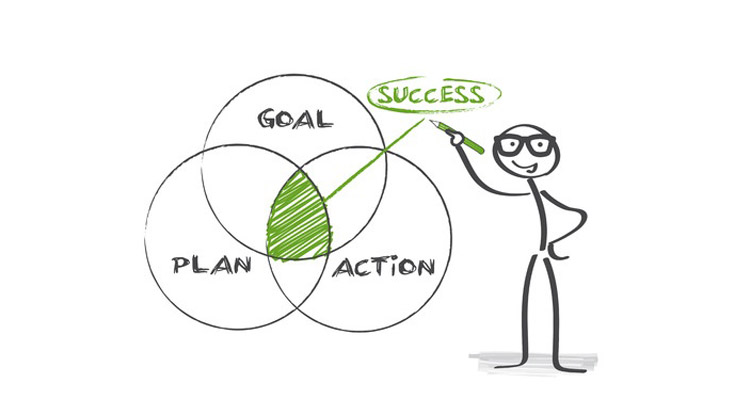
\includegraphics[width=1\textwidth]{immagini/success.jpg}
        \caption{\textit{Goal}}
        \textbf{Fonte}:
        \href{https://brooksplanning.wordpress.com/2016/06/12/action-plan-for-success/
}{brooksplanning.wordpress.com}
        \label{fig: Goal}
    \end{figure}

\newpage

\section{Conoscenze e abilità acquisite}
Questa esperienza si è rivelata molto positiva anche sotto il punto di vista delle conoscenze e competenze che ho acquisito durante i due mesi di stage.
Queste non si limitano solo all'ambito prettamente tecnico ma riguardano anche la realtà aziendale. 
\subsubsection{Azienda}
Ho appreso come un'azienda caratterizza i clienti che utilizzano i suoi prodotti, un aspetto fondamentale dal punto di vista commerciale poiché per creare \textit{software} di successo è necessario che questo abbia dei clienti che lo utilizzino nel tempo. Inoltre ho preso parte ad un contesto aziendale che porta avanti la filosofia del \textit{software} \textit{\gls{opensg}} ed è stato molto interessante vederne le dinamiche. \\
Questo aspetto ha senza dubbio influito sulla scelta del protocollo da utilizzare, in quanto durante lo studio individuale descritto nella sezione \secref{sec:att_analisi}, ho dovuto escludere alcune soluzioni in quanto non compatibili dal punto di vista del tipo di licenza.

\subsubsection{Team di sviluppo}
Ho avuto inoltre modo di lavorare con un \textit{team} di sviluppo completo e di poter collaborare anche con altri reparti dell'azienda che si occupavano di aspetti talvolta distanti dallo sviluppo \textit{software}. Ciò mi ha portato a dover impiegare il giusto linguaggio per comunicare con persone che hanno un punto di vista sul prodotto differente dal mio. \\
Sono rimasto anche sorpreso dal fatto che, nonostante la mia inesperienza, uno dei \textit{senior developer} del \textit{team} mi ha chiesto diverse volte un parere su come avremmo potuto implementare una certa funzionalità. Ciò mi ha fatto comprendere che, nella risoluzione di problemi è molto utile avere diversi pareri pur avendo acquisito un'esperienza considerevole.

\subsubsection{Linguaggi e tecnologie}
Dal punto di vista tecnico ho acquisito alcune conoscenze di cui mi ritengo soddisfatto. Innanzitutto ho potuto osservare e, in parte, mettere in azione in modo professionale alcune tecniche per l'utilizzo di un linguaggio di programmazione (\textit{Java}) da me conosciuto in ambito accademico.
Inoltre ho compreso i vantaggi e le potenzialità di \textit{Docker}, una tecnologia che negli ultimi anni si è ampiamente diffusa sul mercato. \\
Dal punto di vista aziendale mi sono reso conto che le tecnologie vengono sfruttate in tutti i modi possibili per poter raggiungere gli obiettivi. Infatti nel loro impiego può capitare di essere costretti a trovare il giusto compromesso, per esempio tra \textit{performance} e qualità del codice.

\subsubsection{Strumenti}
Ho visto in prima persona come avviene la gestione di un progetto costituito da molte parti e sviluppato da \textit{team} diversi. In particolare l'utilizzo di strumenti di coordinamento come \textbf{Jira} per la gestione di progetto e \textbf{Confluence} per la gestione della documentazione aziendale. \\
Inoltre ho appreso molto dagli sviluppatori \textit{senior} del \textit{team}, i quali mi hanno mostrato come sfruttare al meglio e in modo professionale gli strumenti di sviluppo, al fine di incrementare la produttività e risparmiare tempo.

\subsubsection{Metodo di lavoro}
Oltre ai metodi di lavoro messi in atto dall'azienda, ho potuto sperimentare come condurre la ricerca e lo studio di nuovi argomenti, nel mio caso i protocolli, e come gestire il tempo a disposizione. Tuttavia su questo aspetto ho capito che devo migliorare il mio metodo in quanto, nonostante abbia raggiunto gli obiettivi, non era adeguato per un'analisi approfondita di ciò che stavo studiando. Infatti dopo aver terminato questa attività ho dovuto rivedere alcuni concetti che non avevo ancora compreso completamente.
%**************************************************************
\section{Valutazione personale}
Questa esperienza mi ha fatto riflettere sulla relazione tra il mondo accademico e quello del lavoro. Tutto sommato ritengo che le nozioni apprese durante il corso di laurea triennale siano state molto utili durante questa esperienza, seppur non sufficienti per certi aspetti. \\
Credo che questo meccanismo sia abbastanza naturale poiché l'obiettivo dell'università è quello di erogare conoscenze soprattutto teoriche, necessarie per poter mettere in pratica dei concetti in modo consapevole. Inoltre, essendo il mondo dell'informatica molto ampio, non è pensabile si esplorarlo in soli tre anni. \\
Tuttavia, l'informatica è un campo molto dinamico, cresce e muta anno dopo anno portando alla luce nuovi metodi e tecnologie. Per questo motivo credo che l'offerta didattica erogata dai corsi universitari debba essere adeguatamente aggiornata per poter offrire dei contenuti che siano in linea con ciò che viene utilizzato in ambito professionale. %Inoltre ho notato che molto spesso, quando viene insegnato un linguaggio o una tecnologia, capita che alcune soluzioni vengano etichettate come non ottimali, quando in realtà esistono dei casi d'uso specifici che vengono soddisfatti tramite l'applicazione di tali metodi.
Inoltre avrei preferito che alcuni corsi proponessero degli esempi meno didattici e più concreti, al fine di rendere l'apprendimento più coinvolgente ed efficace. \\
Un modello di insegnamento che ho avuto modo di sperimentare durante questi tre anni, puntava sul fare in modo che lo studente avesse la possibilità di consolidare le conoscenze teoriche con l'ausilio di un progetto didattico significativo, cercando di diminuire il divario tra le conoscenze teoriche e le applicazioni pratiche. In questo caso per esempio, studiare la teoria limitandosi a leggere informazioni presenti nei libri di testo più comuni non era sufficiente, ma era necessario contestualizzarla nell'esperienza vissuta durante il progetto. Nel mio caso, questo metodo è estremamente efficace perché permette di comprendere a fondo i concetti, rendendo quindi poco interessante "ricordare" il loro significato. \\
Nel complesso sono comunque soddisfatto di ciò che mi ha dato l'università, poiché mi ha messo di fronte a nozioni e argomenti che da solo non avrei mai esplorato, anche perché spesso molti aspetti teorici vengono ignorati in campo pratico. In questo modo ho compreso che il modo migliore di risolvere problemi, talvolta complessi, sia quello di unire teoria e pratica in modo strategico. Chiaramente dopo questa esperienza sarò più aperto ad una esplorazione più ampia del mondo dell'informatica, anche dopo aver terminato gli studi. \\
L'attività di stage mi ha pienamente convinto e la consiglio a tutti coloro che hanno la possibilità di farlo, svolto anche in modalità diverse dalla mia, perché è importante per far capire allo studente cosa aspettarsi dal mondo del lavoro e per avere un'idea della tipologia di azienda in cui vuole lavorare.
